\documentclass[tikz,border=1pt]{standalone}

\begin{document}

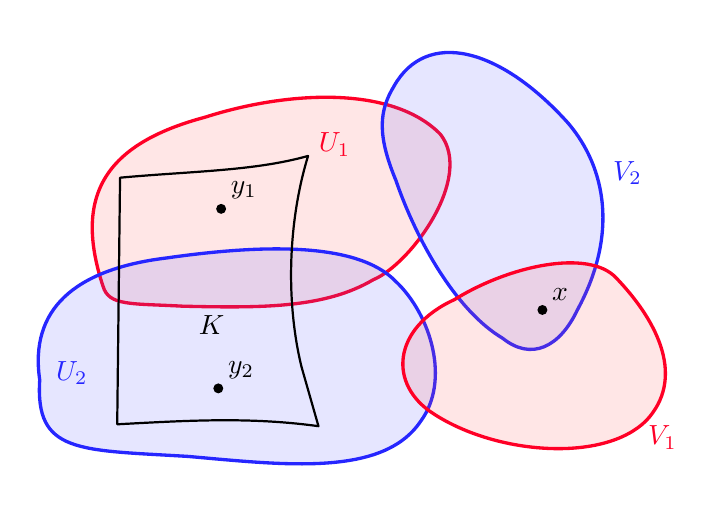
\begin{tikzpicture}[
    line cap=round,
    line join=round,
    scale=1.2,
    redset/.style={
        draw=red!85!magenta,
        line width=1.2pt,
        fill=red!65,
        fill opacity=0.15
    },
    blueset/.style={
        draw=blue!85,
        line width=1.2pt,
        fill=blue!65,
        fill opacity=0.15
    },
    greenset/.style={
        draw=green!65!black,
        line width=2.5pt
    }
]

% -------------------------------------------------
% U_1: red open neighbourhood of y_1
% -------------------------------------------------

\path[redset]
    (2.20,2.35)
    .. controls (1.88,3.32) and (2.23,3.86)
        .. (3.28,4.14)
    .. controls (4.12,4.41) and (5.25,4.49)
        .. (5.77,3.96)
    .. controls (6.13,3.50) and (5.45,2.58)
        .. (5.06,2.42)
    .. controls (4.55,2.12) and (3.90,2.12)
        .. (3.04,2.14)
    .. controls (2.50,2.17) and (2.26,2.14)
        .. cycle;

% -------------------------------------------------
% U_2: blue open neighbourhood of y_2
% -------------------------------------------------

\path[blueset]
    (1.53,1.36)
    .. controls (1.42,2.10) and (1.89,2.53)
        .. (2.87,2.65)
    .. controls (3.85,2.79) and (4.89,2.83)
        .. (5.30,2.40)
    .. controls (5.67,2.05) and (5.88,1.35)
        .. (5.56,0.92)
    .. controls (5.16,0.33) and (4.12,0.46)
        .. (3.10,0.55)
    .. controls (1.94,0.62) and (1.48,0.58)
        .. (1.53,1.36)
    -- cycle;

% -------------------------------------------------
% V_2: blue open neighbourhood of x
% -------------------------------------------------

\path[blueset]
    (5.28,4.47)
    .. controls (5.62,5.07) and (6.39,4.89)
        .. (7.12,4.08)
    .. controls (7.53,3.60) and (7.65,2.89)
        .. (7.22,2.10)
    .. controls (7.03,1.70) and (6.73,1.56)
        .. (6.43,1.80)
    .. controls (5.94,2.09) and (5.52,2.83)
        .. (5.30,3.47)
    .. controls (5.10,3.95) and (5.12,4.21)
        .. cycle;

% -------------------------------------------------
% V_1: red open neighbourhood of x
% -------------------------------------------------

\path[redset]
    (5.70,1.00)
    .. controls (5.21,1.31) and (5.26,1.91)
        .. (5.92,2.21)
    .. controls (6.50,2.57) and (7.34,2.75)
        .. (7.63,2.44)
    .. controls (8.09,1.96) and (8.36,1.37)
        .. (7.95,0.93)
    .. controls (7.50,0.48) and (6.36,0.57)
        .. (5.70,1.00)
    -- cycle;

% -------------------------------------------------
% Green boundary: U_1 union U_2
% -------------------------------------------------

% \draw[greenset]
%     (2.17,2.34)
%     .. controls (1.92,3.00) and (2.25,3.73)
%         .. (3.24,4.10)
%     .. controls (4.20,4.43) and (5.23,4.42)
%         .. (5.71,3.91)
%     .. controls (6.00,3.54) and (5.56,2.82)
%         .. (5.18,2.54)
%     .. controls (5.65,2.15) and (5.90,1.44)
%         .. (5.56,0.98)
%     .. controls (5.14,0.35) and (4.16,0.48)
%         .. (3.03,0.58)
%     .. controls (1.93,0.68) and (1.48,0.68)
%         .. (1.54,1.37)
%     .. controls (1.55,1.93) and (1.71,2.16)
%         .. (2.17,2.34);

% -------------------------------------------------
% Green region: V_1 intersection V_2
% -------------------------------------------------

% \path[
%     fill=green!60,
%     fill opacity=0.35,
%     draw=green!65!black,
%     line width=2.5pt
% ]
%     (6.35,2.25)
%     .. controls (6.75,2.50) and (7.06,2.56)
%         .. (7.25,2.59)
%     .. controls (7.38,2.18) and (7.28,1.89)
%         .. (7.05,1.73)
%     .. controls (6.80,1.60) and (6.50,1.70)
%         .. (6.35,2.25)
%     -- cycle;

% -------------------------------------------------
% Compact set K (black outline)
% -------------------------------------------------

\draw[black,thick]
    (2.35,0.89)
    -- (2.38,3.50)
    .. controls (3.15,3.57) and (3.80,3.57)
        .. (4.37,3.73)
    .. controls (4.16,3.05) and (4.13,2.20)
        .. (4.30,1.50)
    -- (4.48,0.87)
    .. controls (3.75,0.97) and (3.10,0.93)
        .. (2.35,0.89);

% -------------------------------------------------
% Points y_1, y_2 in K
% -------------------------------------------------

\fill[black] (3.45,3.17) circle (1.5pt);
\node[above right] at (3.45,3.17) {$y_1$};

\fill[black] (3.42,1.27) circle (1.5pt);
\node[above right] at (3.42,1.27) {$y_2$};

\node at (3.35,1.94) {$K$};

% -------------------------------------------------
% Point x in V_1 intersection V_2
% -------------------------------------------------

\fill[black] (6.85,2.10) circle (1.5pt);
\node[above right] at (6.85,2.10) {$x$};

% -------------------------------------------------
% Labels
% -------------------------------------------------

\node[red!85!magenta] at (4.65,3.85) {$U_1$};
\node[blue!85] at (1.87,1.43) {$U_2$};

\node[blue!85] at (7.75,3.55) {$V_2$};
\node[red!85!magenta] at (8.12,0.75) {$V_1$};

\end{tikzpicture}

\end{document}